% Paper 2 (academic structure). IEEE BigData 2026 workshop (4th Int. Workshop on Trustworthy and Aligned AI),
% 10 pages including references. Same study, data and numbers as paper 1 (IEEE_BigData2026_paper/).
% Protocol frozen 2026-11-12 02:16 CST (hash 22d4f2fa...); registered on OSF (osf.io/bn6va).
\documentclass[conference]{IEEEtran}
\IEEEoverridecommandlockouts
\usepackage{iftex}
\ifXeTeX % Tectonic/XeLaTeX build: use a Times clone so the layout matches pdfLaTeX + IEEEtran
  \usepackage{fontspec}
  \setmainfont{texgyretermes}[Extension=.otf, UprightFont=*-regular, BoldFont=*-bold,
    ItalicFont=*-italic, BoldItalicFont=*-bolditalic]
\fi
\usepackage{cite}
\usepackage{amsmath,amssymb}
\usepackage{graphicx}
\usepackage{booktabs}
\usepackage{array}
\usepackage{xcolor}
\usepackage{url}
\usepackage{tikz}
\usetikzlibrary{positioning,arrows.meta,fit,calc}
\usepackage{algorithm}
\usepackage{algpseudocode}
\usepackage[hidelinks]{hyperref}

\newcommand{\vcr}{\mathrm{VCR}}
\newcommand{\sys}[1]{\textsf{#1}}

\begin{document}

\title{Do LLM Agents Verify Their Data?\\ Available vs.\ Enforced Checks in Data Mining}

\author{\IEEEauthorblockN{Ahsan Shahid, Mohammed Muzakkiruddin Ahmed, Hadi Rashid, Abdelrahman Elfikky, and John R. Talburt}
\IEEEauthorblockA{\textit{Department of Computer Science, University of Arkansas at Little Rock}, Little Rock, AR, USA\\
\{axshahid, mmohammed6, harashid, aelfikky1, jrtalburt\}@ualr.edu}}

\maketitle

\begin{abstract}
Large language model (LLM) agents are increasingly used to build data-mining pipelines, but a pipeline can score well
while it reads a tampered file, drops records, or mixes up units. We study whether such agents check their data when
a verifying tool is available, and what changes when checks are enforced. We designed a controlled benchmark of 36
classification and regression tasks from six dataset families with declared and hidden data defects, scored by an
independent evaluator, and compared seven systems with the same tools and budgets: a rule-based workflow, a single
agent, and a three-agent team, each with and without quality and provenance checks. The protocol was frozen before
the evaluation runs and registered. In 8,352 runs, agents without enforced checks rarely verified: on silently changed
data they used the hash-verifying load in 1 and 12 of 108 runs, about as often as when nothing was wrong, against
104--107 of 108 when the check was enforced. Enforcement fixed that defect, but one range check also rejected correct
data in 2 of 18 blocks, where every system using it failed. The primary hypothesis, that a fully checked team
outperforms an unchecked one, was not supported ($+0.1$ points, 95\% CI $-11.1$ to $+9.9$). A team did not beat a
single agent, and a second model showed the same pattern. Verification that is only available is rarely used, and an
enforced check is only as good as its rule.
\end{abstract}

\begin{IEEEkeywords}
data mining, data quality, data provenance, LLM agents, verification, benchmark, multi-agent systems
\end{IEEEkeywords}

% =====================================================================
\section{Introduction}
% =====================================================================
Data mining turns raw records into models and decisions, and its results are only as good as the data behind them.
LLM agents can now carry out much of this work themselves: they find the tables, clean and join them, fit a model, and
submit predictions. This promises faster analysis, but it also moves data handling out of sight. A pipeline can
reach a good test score while it has read an outdated or tampered file, dropped or duplicated records, or converted
units wrongly. In applied machine learning, errors of this kind, data leakage in particular, have already caused
widespread failures to reproduce published results~\cite{kapoor2023leakage}.

Benchmarks for data-science agents mostly score the final answer. On them the best agents solve 34\% of DSBench
analysis tasks~\cite{jing2025dsbench}, 15\% of the hard DABstep tasks~\cite{egg2025dabstep}, and 57\% of Data Agent
Benchmark queries~\cite{ma2026dab}. Whether the data were handled correctly is not measured. Two remedies are usually
proposed: let agents check their own work, and split the work across a team of specialised agents. LLMs correct
themselves poorly without outside feedback~\cite{huang2024selfcorrect} but better with feedback from
tools~\cite{gou2024critic}, which favours checks that are executed rather than judged.

Consider a concrete case. A source file is silently replaced: its catalog entry still lists the authorised version and
hash, but the stored content has changed, and the values still look plausible. An agent can detect this only by
recomputing the content hash, an operation it has but does not have to use. Does it? And if a check is enforced
before submission, does the pipeline become more reliable, or can the check itself get in the way? We address these
questions with four research questions:
\begin{itemize}
\item \textbf{RQ1.} Do LLM agents use an available verification operation when nothing forces them to?
\item \textbf{RQ2.} Does enforcing quality and provenance checks increase the share of correctly verified
pipelines? (primary hypothesis H1)
\item \textbf{RQ3.} What does each type of check contribute, and on which defects? (H2)
\item \textbf{RQ4.} At equal budgets, does a team of agents outperform a single agent (H3), and do agents outperform
a rule-based workflow (H4)?
\end{itemize}

To answer them we built a benchmark and a frozen experimental protocol (Section~\ref{sec:method}). Our development
pilots shaped the design: when each defect and its remedy were written into the task, every system, including the
rule-based workflow, solved 95--100\% of the tasks, so we added defects that break a stated requirement without being
described. This paper makes three contributions.
(1)~A data-mining benchmark with declared and hidden defects, a hidden record of every injected change, an oracle
solver checked on every hidden-defect instance, and an independent evaluator that scores how the data were handled.
(2)~A formal model and a budget-matched experimental design that separate who plans the work from which checks are
enforced, with the verifying operation available to every system.
(3)~Evidence from 8,352 runs under a protocol frozen before the evaluation runs, answering RQ1--RQ4, including a
null primary result and a failure mode of enforced checks.

% =====================================================================
\section{Literature Review}
\label{sec:related}
% =====================================================================
\subsection{Benchmarks for data-science agents}
Several benchmarks measure how well LLM agents perform data analysis and machine learning. InfiAgent-DABench turns
open data-analysis questions into automatically scored ones~\cite{hu2024infiagent}; DSBench combines data-analysis and
modelling tasks from real competitions~\cite{jing2025dsbench}; MLE-bench compares agents with human Kaggle
leaderboards~\cite{chan2025mlebench}; DABstep~\cite{egg2025dabstep}, Spider~2.0~\cite{lei2025spider2}, and
DAB~\cite{ma2026dab} target multi-step analytics, enterprise SQL, and heterogeneous databases. Agent systems such as
DS-Agent~\cite{guo2024dsagent}, Data Interpreter~\cite{hong2024datainterpreter}, and DS-STAR~\cite{nam2025dsstar}
add case-based planning, task graphs, and an LLM verifier. These works established that agents can complete realistic
data tasks and measured how often they succeed. Li et~al.\ audited agentic data-science solutions and found that
most contained a methodological failure such as leakage or inappropriate validation~\cite{li2026silent}, which shows
that scoring the final answer is not enough. Our benchmark builds on this line by scoring explicit data-handling
properties of the submitted workflow.

\subsection{Data quality, cleaning, and provenance}
Data validation before training and serving is standard in production machine learning~\cite{polyzotis2019datavalidation},
and data-quality verification has been automated at scale~\cite{schelter2018deequ}. Data dependencies are a known
source of technical debt~\cite{sculley2015debt}, and mlinspect detects distribution problems introduced by pipeline
steps~\cite{grafberger2021mlinspect}. HoloClean showed how holistic repair improves data quality~\cite{rekatsinas2017holoclean}.
Provenance models represent sources as entities and transformations as activities~\cite{w3c2013provdm}, and Vamsa
infers provenance from data-science scripts~\cite{namaki2020vamsa}. With LLM agents, DataGovBench evaluates
data-governance tasks~\cite{liu2025datagovbench}, a study of reference-free agentic cleaning found that a
deterministic profiling baseline detected errors best~\cite{fadlallah2026cleaning}, multi-agent debate helped error
detection when grounded in code execution~\cite{parmar2026debate}, and agent-generated validation rules can be vetted
before execution~\cite{fadlallah2026dqa}. We use quality and provenance checks of this kind as treatments that an agent
does or does not receive.

\subsection{Single agents, teams, and budgets}
Tool-using agents interleave reasoning with actions~\cite{yao2023react}, and multi-agent frameworks assign roles to
several such agents~\cite{wu2023autogen,hong2024metagpt}. Controlled comparisons find that teams rarely beat a single
agent once compute is matched~\cite{tran2026single,fu2026moreagents,dylan2026equalcost,jwalapuram2026illusion}, that
the benefit of coordination depends on task structure~\cite{kim2025scaling}, and that task verification is one of the
main groups of multi-agent failures~\cite{cemri2025mas}. We extend these comparisons to data mining and add enforced
checks as a second factor.

\subsection{Available versus enforced verification}
The closest studies, all from 2026, ask whether agents use checks. SARC-DQ found that a metadata-aware gate recovered
losses from metadata-borne defects such as stale records that stronger models did not~\cite{besanson2026sarcdq}, and composed gates can
interfere with each other~\cite{besanson2026onegate}. LIMBO showed that tool contracts decide whether agents avoid
duplicated side effects~\cite{li2026limbo}. RITE identified using an available verification path as one of the
bottlenecks in handling silent tool errors~\cite{zhang2026rite}. In coding, completion gates and independent review
outperformed instructions~\cite{zhang2026rethinking}, and executable guardrails raised constraint compliance on
SWE-bench Lite from 67.0\% to 88.3\%~\cite{sharma2026contextcov}. Verification prompts reduced reliance on corrupted
tool outputs~\cite{yang2026overreliance}, and tool use depends strongly on how tools are
described~\cite{faghih2025toolprefs}. On benchmark design, the Agentic Benchmark Checklist recommends verifying that
each task is solvable~\cite{zhu2025abc}, and execution-based scoring follows SWE-bench~\cite{jimenez2024swebench}.

\subsection{Research gap}
These studies show, in coding, tool use, and operations, that agents often skip available checks and that enforced
checks help. Based on their published descriptions, none combines (i)~data-mining tasks scored on data handling
rather than final answers, (ii)~a verifying operation documented identically to every system, so that available and
enforced verification can be compared directly, (iii)~a rule-based baseline and single and multi-agent systems under
matched budgets, and (iv)~a protocol frozen before the evaluation runs. This study fills that gap.

% =====================================================================
\section{Methodology}
\label{sec:method}
% =====================================================================
\subsection{Research design and why it was chosen}
We use a controlled, paired experiment. Every system runs on exactly the same task instances, with the same tools,
candidate models, and resource budget, so differences in outcome can be attributed to the system design and not to
the task, the data, or extra compute. This design suits our questions because each research question is a
comparison between system designs (with versus without checks, team versus single agent). We fixed the hypotheses,
analysis plan, and resource limits before the evaluation runs and stored them in a hashed record, following the logic
of preregistration, which separates confirmatory tests from exploratory findings~\cite{nosek2018prereg}. The record
was registered on OSF. The outcome is scored by software only, without LLM or human grading, so that the measurement
cannot depend on the systems being measured.

\subsection{Benchmark and datasets}
\label{sec:bench}
Table~\ref{tab:data} lists the six dataset families. D1--D4 are public UCI datasets under CC~BY~4.0, chosen because
they are well documented and widely used for classification and regression; AI4I~2020 is itself
synthetic~\cite{matzka2020ai4i}, and the Energy Efficiency data describe simulated buildings~\cite{tsanas2012energy}.
D5 and D6 are relational datasets from seeded generators, added so that some tasks cannot have appeared in model
training data. Six task templates per family give 36 tasks: single-source modelling (T1), two- and three-table
integration (T2, T3), harmonising documented unit representations (T4), choosing the authorised version of a source
(T5), and computing per-record aggregates from child readings (T6). Each table is split into 20 shards per partition.
Every system receives the same task contract: target, allowed and excluded features, source versions, keys, units,
aggregation rules, plausible value ranges, and budget.

\begin{table}[t]
\caption{Dataset families}
\label{tab:data}
\centering\footnotesize\setlength{\tabcolsep}{4pt}
\begin{tabular}{@{}llrl@{}}
\toprule
ID & Source & Rows & Target \\
\midrule
D1 & AI4I 2020~\cite{uci601ai4i} & 10,000 & failure (binary) \\
D2 & Steel Plates Faults~\cite{uci198steel} & 1,941 & fault (7 classes) \\
D3 & Concrete Strength~\cite{uci165concrete,yeh1998concrete} & 1,030 & strength (regression) \\
D4 & Energy Efficiency~\cite{uci242energy} & 768 & heating load (regr.) \\
D5 & Synthetic machinery & 10,000 & failure (binary) \\
D6 & Synthetic process & 9,000 & output (regression) \\
\bottomrule
\end{tabular}
\end{table}

\textbf{Defects.} Tier~1 defects are declared in the contract together with their remedy: missing or string-encoded
numbers (5\% or 20\% of cells), duplicated or aliased keys (5\% or 20\%), and changed representations or stale
sources (a quarter of the shards), plus a clean condition. Tier~2 defects break a requirement that the contract states
but are not described (Table~\ref{tab:tier2}): key variants that break record matching (X2), shards in an undeclared
unit representation (X3), and content drift (X4), where an authorised file was silently replaced while its catalog
entry still lists the authorised hash and a correct replica exists. X4 values stay plausible, so the only reliable
way to detect it is to recompute content hashes. Each Tier~2 defect can be repaired by a general operation that is
documented to every system in both tiers. Its severity was chosen in the pilots by a rule fixed in advance (the level
whose baseline success rate is closest to 0.5).

\begin{table}[t]
\caption{Tier~2 defects (frozen level in bold)}
\label{tab:tier2}
\centering\footnotesize\setlength{\tabcolsep}{3pt}
\begin{tabular}{@{}lp{0.27\columnwidth}p{0.25\columnwidth}l@{}}
\toprule
ID & Levels & Detected by & Repair \\
\midrule
X2 & 5\% / \textbf{10\%} / 20\% of keys & record coverage (Q) & \texttt{\scriptsize normalize\_key} \\
X3 & \textbf{1} / 2 / 4 of 20 shards & value ranges (Q) & \texttt{\scriptsize infer\_representation} \\
X4 & 1 / \textbf{2} / 4 of 20 shards & content hash (P) & \texttt{\scriptsize authoritative\_verified} \\
\bottomrule
\end{tabular}
\end{table}

\textbf{Evaluator and solvability.} The generator records every injected change outside the agents' environment. An
independent evaluator, running in a separate process, replays the submitted workflow on hidden test data and checks
that the target, source authority, excluded features, records, joins, units, and aggregates match an independent
reference (absolute tolerance $10^{-8}$, relative $10^{-6}$), that preprocessing was fitted on training data only,
and that every hidden record gets a valid prediction. Fixtures with known verdicts tested the evaluator before any
run. Following the Agentic Benchmark Checklist~\cite{zhu2025abc}, an oracle solver had to reproduce the hidden
reference on every Tier~2 instance; it did so on all 324 formal instances before the protocol was frozen.

\subsection{Systems compared}
\label{sec:systems}
Table~\ref{tab:systems} lists the seven systems. \sys{F} is a rule-based workflow written from the declared
specification; it represents strong conventional automation. The agents follow the tool-use loop of
ReAct~\cite{yao2023react}: a single agent (\sys{S}), or a three-role team (\sys{M}) in which a coordinator delegates
to a data manager and a mining agent through a shared blackboard~\cite{wu2023autogen,hong2024metagpt}. All act only
through the same bounded tools: listing, inspecting, profiling, and read-only querying of sources (in-memory
DuckDB~\cite{raasveldt2019duckdb}); \texttt{materialize\_features}, which executes a validated declarative graph of
operations (load, parse, convert units, map aliases, normalise keys, infer representation, de-duplicate, join,
aggregate); \texttt{fit\_evaluate} over six fixed scikit-learn pipelines~\cite{pedregosa2011sklearn}; \texttt{submit};
and \texttt{abstain}. The \emph{quality gate} (Q) checks required columns, excluded features, key uniqueness, record
coverage, value ranges, unit conversion, and aggregates, in the spirit of production data
validation~\cite{polyzotis2019datavalidation,schelter2018deequ}. The \emph{provenance gate} (P) checks source
authority, versions, recomputed content hashes, column lineage, and that models were fitted on training data only,
following provenance models~\cite{w3c2013provdm}. In gated systems, verdicts are returned to the agent and a failing
gate blocks submission; ungated systems see only ordinary tool output. ``Enforced'' therefore means enforced with
feedback. Fig.~\ref{fig:arch} shows the architecture.

\begin{table}[t]
\caption{Systems. All share the data tools, candidate models, and budgets; gated systems also have two check tools.}
\label{tab:systems}
\centering\footnotesize\setlength{\tabcolsep}{5pt}
\begin{tabular}{@{}lllcc@{}}
\toprule
System & Planning & LLM & Quality gate & Provenance gate \\
\midrule
\sys{F}   & rule-based workflow & no  & yes & yes \\
\sys{S0}  & single agent        & yes & --  & -- \\
\sys{SQP} & single agent        & yes & yes & yes \\
\sys{M0}  & three-role team     & yes & --  & -- \\
\sys{MQ}  & three-role team     & yes & yes & -- \\
\sys{MP}  & three-role team     & yes & --  & yes \\
\sys{MQP} & three-role team     & yes & yes & yes \\
\bottomrule
\end{tabular}
\end{table}

\begin{figure*}[t]
\centering
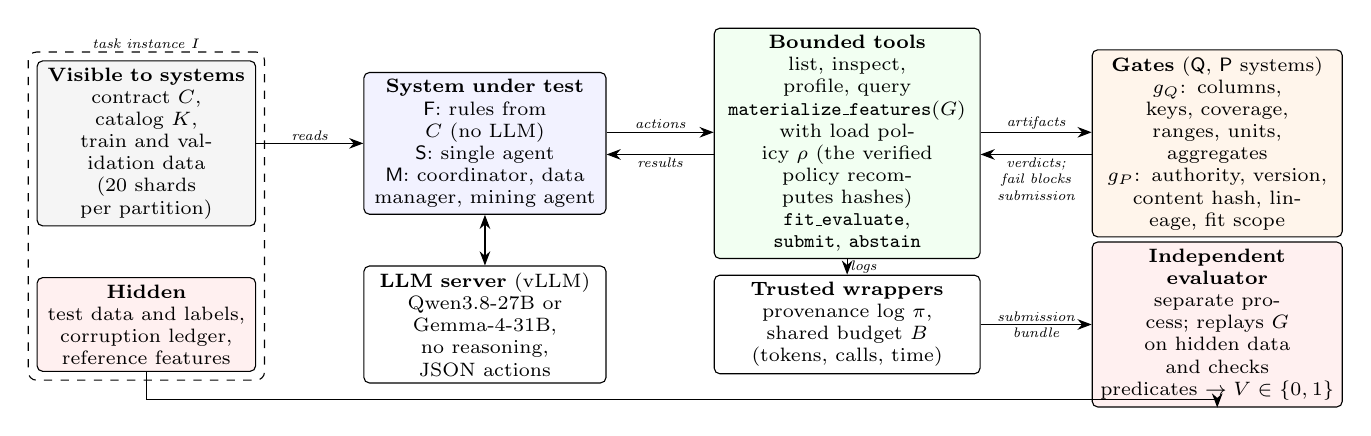
\begin{tikzpicture}[font=\scriptsize, >={Stealth[length=1.8mm]},
  box/.style={draw, rounded corners=2pt, align=center, inner sep=2.5pt},
  grp/.style={draw, dashed, rounded corners=3pt, inner sep=3pt},
  lab/.style={font=\tiny\itshape, inner sep=1pt, align=center}]
\node[box, text width=2.6cm, fill=gray!8] (vis) at (0,1.0) {\textbf{Visible to systems}\\ contract $C$, catalog $K$,\\ train and validation data\\ (20 shards per partition)};
\node[box, text width=2.6cm, fill=red!6] (hid) at (0,-1.3) {\textbf{Hidden}\\ test data and labels,\\ corruption ledger,\\ reference features};
\node[grp, fit=(vis)(hid), label={[lab]above:task instance $I$}] (inst) {};
\node[box, text width=2.9cm, fill=blue!5] (sys) at (4.3,1.0) {\textbf{System under test}\\ \sys{F}: rules from $C$ (no LLM)\\ \sys{S}: single agent\\ \sys{M}: coordinator, data\\ manager, mining agent};
\node[box, text width=2.9cm] (llm) at (4.3,-1.3) {\textbf{LLM server} (vLLM)\\ Qwen3.8-27B or Gemma-4-31B,\\ no reasoning, JSON actions};
\node[box, text width=3.2cm, fill=green!5] (tools) at (8.9,1.0) {\textbf{Bounded tools}\\ list, inspect, profile, query\\ \texttt{materialize\_features}($G$)\\ with load policy $\rho$ (the verified\\ policy recomputes hashes)\\ \texttt{fit\_evaluate}, \texttt{submit}, \texttt{abstain}};
\node[box, text width=3.2cm] (wrap) at (8.9,-1.3) {\textbf{Trusted wrappers}\\ provenance log $\pi$,\\ shared budget $B$\\ (tokens, calls, time)};
\node[box, text width=3.0cm, fill=orange!8] (gates) at (13.6,1.0) {\textbf{Gates} (\sys{Q}, \sys{P} systems)\\ $g_Q$: columns, keys, coverage,\\ ranges, units, aggregates\\ $g_P$: authority, version,\\ content hash, lineage, fit scope};
\node[box, text width=3.0cm, fill=red!6] (eval) at (13.6,-1.3) {\textbf{Independent evaluator}\\ separate process; replays $G$\\ on hidden data and checks\\ predicates $\to V\in\{0,1\}$};
\draw[->] (vis) -- node[lab,above]{reads} (sys);
\draw[->] ([yshift=4pt]sys.east) -- node[lab,above]{actions} ([yshift=4pt]tools.west);
\draw[<-] ([yshift=-4pt]sys.east) -- node[lab,below]{results} ([yshift=-4pt]tools.west);
\draw[<->] (sys) -- (llm);
\draw[->] (tools) -- node[lab,right]{logs} (wrap);
\draw[->] ([yshift=4pt]tools.east) -- node[lab,above]{artifacts} ([yshift=4pt]gates.west);
\draw[<-] ([yshift=-4pt]tools.east) -- node[lab,below]{verdicts;\\ fail blocks\\ submission} ([yshift=-4pt]gates.west);
\draw[->] (wrap) -- node[lab,above]{submission} node[lab,below]{bundle} (eval);
\draw[->] (hid.south) -- ++(0,-0.35) -| (eval.south);
\end{tikzpicture}
\caption{Architecture. Every system acts only through the same bounded tools on the visible part of a task instance.
Trusted wrappers record provenance and charge one shared budget. In gated systems, gate verdicts are returned to the
agent and a failing gate blocks submission. Only the independent evaluator sees the hidden data; it replays the
submitted workflow and returns the verified-completion outcome $V$.}
\label{fig:arch}
\end{figure*}

\subsection{Formal model and algorithm}
A task instance is $I=(C,K,D,H)$: a contract $C$, a catalog $K$ of candidate files with declared versions and SHA-256
hashes, visible data $D$ (train and validation), and hidden data $H$ (test partition, labels, ledger, reference). A
system submits a workflow $(G,m)$, a declarative graph $G$ and one of the six candidate models $m$, or abstains. Each
\texttt{load} node names a table and a policy $\rho$. For an authority record with version $v^\star$ and shard hashes
$h^\star_s$, \texttt{authoritative} selects for each shard $s$ a file $f$ with $v(f)=v^\star$ and declared hash
$h_s(f)=h^\star_s$; \texttt{authoritative\_verified} additionally requires $\mathrm{SHA256}(f_s)=h^\star_s$, the hash of
the content actually stored. A gate is a vector of predicates $g(G,D,\pi)\in\{0,1\}^{k}$ over the materialised data
and the trusted provenance log $\pi$. A system with gate set $S\subseteq\{Q,P\}$ may submit only if
\begin{equation}
\textstyle\bigwedge_{g\in S}\bigwedge_{j} g_j(G,D,\pi)=1;
\label{eq:gate}
\end{equation}
otherwise the failing checks are returned and the agent may repair (at most $R=2$ times) or abstain. The run ends on
submission, abstention, or when the budget $B$ (tokens, model calls, tool calls, active time) is spent. The outcome is
verified completion,
\begin{equation}
V(I,G,m)=\textstyle\prod_{j}\phi_j(G,m;H)\in\{0,1\},
\label{eq:v}
\end{equation}
the product of the evaluator's predicates $\phi_j$, evaluated by replaying $G$ on $H$; abstentions and exhausted
budgets count as $V=0$. Verification uptake of system $s$ under condition $c$ is
$U_s(c)=\Pr[\,\exists\,\texttt{load}\in G:\rho=\texttt{authoritative\_verified}\mid s,c\,]$, over every graph the run
passed to \texttt{materialize\_features}. Algorithm~\ref{alg:run} gives one agentic run. In the team, the coordinator
can also \texttt{delegate} to the data manager or mining agent, who run the same loop for at most 12 steps; every role
is charged to the same budget, and only the coordinator may submit. \sys{F} replaces the LLM with a fixed graph built
from $C$ and $K$ using \texttt{authoritative} loads and the declared repairs, and submits if Eq.~(\ref{eq:gate}) holds
for $S=\{Q,P\}$, otherwise abstains.

\begin{algorithm}[t]
\caption{One agentic run of system $s$ with gate set $S$ on instance $I$}
\label{alg:run}
\footnotesize
\begin{algorithmic}[1]
\State $h\gets$ task text from $C$ and $K$; $r\gets0$; $\textit{failed}\gets\textbf{false}$
\While{budget $B$ not exhausted}
  \State $a\gets\textsc{LLM}(h)$ \Comment{JSON action; 3 invalid in a row end the run}
  \If{$a=\texttt{abstain}(\textit{reason})$} \Return \textsc{Abstained}(\textit{reason}) \EndIf
  \If{$a=\texttt{materialize}(G)$}
    \If{\textit{failed} \textbf{and} $r=R$} $o\gets$ ``repair limit reached''
    \Else
      \If{\textit{failed}} $r\gets r+1$ \EndIf
      \State execute $G$ on $D$; $o\gets$ summaries; \textbf{for} $g\in S$: $o\gets o\cup g(G,D,\pi)$
      \State $\textit{failed}\gets$ execution error or any gate check $=0$
    \EndIf
  \ElsIf{$a=\texttt{submit}(G,m)$}
    \If{Eq.~(\ref{eq:gate}) fails} $o\gets$ failing checks; $\textit{failed}\gets\textbf{true}$
    \Else\ refit $m$ on train and validation; \Return \textsc{Submitted}$(G,m)$
    \EndIf
  \Else\ $o\gets$ result of the read-only tool or \texttt{fit\_evaluate}
  \EndIf
  \State $h\gets h\,\|\,(a,o,\text{remaining }B)$
\EndWhile
\State \Return \textsc{BudgetExceeded}
\end{algorithmic}
\end{algorithm}

\subsection{Experimental setup}
The main model (backbone A) is \texttt{Qwen/Qwen3.8-27B}~\cite{qwen2026qwen38}; the replication uses
\texttt{google/gemma-4-31B-it}~\cite{google2026gemma4} from a second vendor. Both are open models, pinned to fixed
revisions and served with vLLM~\cite{kwon2023vllm} on one NVIDIA RTX PRO 6000 GPU, with temperature 0.2, a
16,384-token context, reasoning mode off, and JSON actions. Each run may use 300,000 tokens, 48 model calls, 40 tool
calls, six model evaluations, two repair cycles, and 600\,s; the token limit came from a rule fixed before the pilots.
The main experiment (E1) runs all seven systems on 36 tasks, ten conditions (C0--C6, X2b, X3a, X4b), and three
repetitions: 7,560 runs. E4 repeats \sys{M0}, \sys{SQP}, and \sys{MQP} with backbone B on six tasks fixed in advance
(540 runs). E5 tests refusal on two unsatisfiable variants, a missing required source (N1) and conflicting authority
records (N2), for all systems (252 runs). E6 replays retained submissions under order changes and corruptions. Run
order is randomised within paired blocks, eight runs execute concurrently, and failed runs are never rerun except
for verified infrastructure failures (ten, retried once).

\subsection{Statistical analysis}
For RQ2--RQ4, the estimate is a paired, family-weighted difference in verified-completion rate: within each family
and repetition we average the paired differences over tasks and conditions, then average over repetitions and the six
families. Uncertainty comes from a block bootstrap with 10,000 draws that resamples repetition blocks within each
family~\cite{efron1979bootstrap,saravanan2020hierarchical}, which respects the pairing and clustering of runs.
$p$ values come from a paired sign-flip test over the 18 family--repetition blocks (10,000 draws, two-sided). H1
(\sys{MQP} versus \sys{M0}) is the only primary hypothesis. The quality and provenance main effects, their
interaction, \sys{MQP}$-$\sys{SQP}, and \sys{MQP}$-$\sys{F} on Tier~1 form a secondary family with Holm
adjustment~\cite{holm1979}. Prespecified sensitivity analyses are a variance-inflated interval, leave-one-family-out
estimates, a mixed-effects logistic model, results by tier, and results without X4. RQ1 is a prespecified descriptive
outcome measured from the trusted traces. Analyses not in the frozen plan are labelled post hoc.

% =====================================================================
\section{Results}
\label{sec:results}
% =====================================================================
All 8,352 scheduled runs were completed. Table~\ref{tab:main} gives the verified-completion rate (VCR) of each system,
Fig.~\ref{fig:main} the main patterns, Table~\ref{tab:contrasts} the tests of the hypotheses, and
Table~\ref{tab:summary} a summary of each research question.

\begin{table}[t]
\caption{Summary of research questions, expectations, and results}
\label{tab:summary}
\centering\footnotesize\setlength{\tabcolsep}{3pt}
\begin{tabular}{@{}p{0.09\columnwidth}p{0.3\columnwidth}p{0.36\columnwidth}p{0.17\columnwidth}@{}}
\toprule
RQ & Expectation (pilots) & Result (E1) & Verdict \\
\midrule
RQ1 & ungated agents rarely verify & 1 and 12 of 108 X4 runs vs.\ 104--107 when enforced & confirmed (descriptive) \\
RQ2 (H1) & gated team beats ungated team & $+0.1$ [$-11.1$, $+9.9$] & not supported \\
RQ3 (H2) & each gate helps on its defects & P: $+6.4$, $p<0.001$, X4 only; Q: $-6.3$, $p=0.50$ & partly supported \\
RQ4 (H3) & no team advantage & team $-3.2$, $p=0.041$ & team worse \\
RQ4 (H4) & no direction & rule-based \sys{F} $+5.4$ over gated team, $p=0.001$ & \sys{F} better \\
\bottomrule
\end{tabular}
\end{table}

\begin{table}[t]
\caption{Verified-completion rate by system (E1, backbone A, 36 tasks, 3 repetitions)}
\label{tab:main}
\centering\footnotesize\setlength{\tabcolsep}{4pt}
\begin{tabular}{@{}lrrrrr@{}}
\toprule
System & Tier 1 & Tier 2 & All & X2, X3 & X4 \\
 & ($n$=756) & ($n$=324) & ($n$=1,080) & ($n$=216) & ($n$=108) \\
\midrule
\sys{F}   & 0.889 & 0.000 & 0.622 & 0.000 & 0.000 \\
\sys{S0}  & 0.958 & 0.429 & 0.799 & 0.639 & 0.009 \\
\sys{M0}  & 0.938 & 0.451 & 0.792 & 0.625 & 0.102 \\
\sys{MQ}  & 0.841 & 0.537 & 0.750 & 0.662 & 0.287 \\
\sys{MP}  & 0.938 & 0.738 & 0.878 & 0.648 & 0.917 \\
\sys{SQP} & 0.858 & 0.747 & 0.825 & 0.704 & 0.833 \\
\sys{MQP} & 0.835 & 0.694 & 0.793 & 0.620 & 0.843 \\
\bottomrule
\end{tabular}
\end{table}

\begin{figure}[t]
\centering
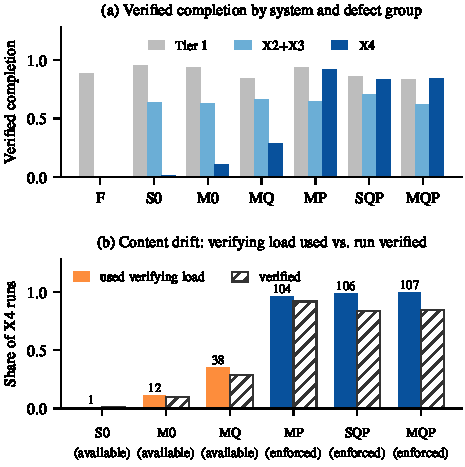
\includegraphics[width=\columnwidth]{figures/fig_main.pdf}
\caption{(a)~Verified completion on declared defects (Tier~1), hidden defects other than content drift (X2, X3), and
content drift (X4). (b)~On X4, the share of runs that used the hash-verifying load, which every system can use, and
the share that were verified; numbers are run counts out of 108.}
\label{fig:main}
\end{figure}

\begin{table*}[t]
\caption{Hypothesis tests (percentage points, family-weighted, 95\% block-bootstrap interval; Holm-adjusted
sign-flip $p$ for the secondary family). ``No X4'': all conditions except content drift.}
\label{tab:contrasts}
\centering\footnotesize\setlength{\tabcolsep}{3pt}
\begin{tabular}{@{}llrrrrr@{}}
\toprule
RQ & Contrast & All (pooled) & Holm $p$ & Tier 1 & Tier 2 & No X4 \\
\midrule
RQ2 & H1: \sys{MQP}$-$\sys{M0} (primary) & $+0.1$ [$-11.1$, $+9.9$] & -- & $-10.3$ [$-21.3$, $-0.7$] & $+24.4$ [$+12.3$, $+34.9$] & $-8.1$ [$-19.1$, $+1.4$] \\
RQ3 & Quality main effect & $-6.3$ [$-17.3$, $+3.8$] & 0.50 & $-10.0$ [$-21.1$, $+0.3$] & $+2.2$ [$-9.0$, $+12.0$] & $-7.7$ [$-18.7$, $+2.4$] \\
RQ3 & Provenance main effect & $+6.4$ [$+5.5$, $+7.4$] & $<$0.001 & $-0.3$ [$-1.2$, $+0.5$] & $+22.2$ [$+19.8$, $+24.7$] & $-0.5$ [$-1.4$, $+0.5$] \\
RQ3 & Quality $\times$ provenance & $-4.4$ [$-6.2$, $-2.5$] & 0.013 & $-0.7$ [$-2.5$, $+1.2$] & $-13.0$ [$-18.5$, $-7.4$] & $-2.0$ [$-3.8$, $-0.2$] \\
RQ4 & H3: \sys{MQP}$-$\sys{SQP} (team vs.\ single) & $-3.2$ [$-4.5$, $-1.8$] & 0.041 & $-2.4$ [$-3.8$, $-0.7$] & $-5.2$ [$-8.0$, $-2.5$] & $-3.7$ [$-5.2$, $-2.0$] \\
RQ4 & H4: \sys{MQP}$-$\sys{F} (Tier~1) & -- & 0.001 & $-5.4$ [$-7.9$, $-2.5$] & -- & -- \\
\bottomrule
\end{tabular}
\end{table*}

\subsection{RQ1: Do agents verify when nothing forces them?}
\textbf{Expectation.} In the pilots, ungated agents rarely used the hash-verifying load (2 and 5 of 72 runs with
content drift), so we expected low uptake.
\textbf{Result.} The expectation held (Fig.~\ref{fig:main}b). On X4 the ungated single agent used the verifying load in
1 of 108 runs and the ungated team in 12, against 104--107 for the systems whose provenance check was enforced. The
ungated agents' use did not respond to the defect: the team used it in 11.1\% of X4 runs and in 13.1\% of Tier~1 runs,
where nothing had changed, and the single agent in 0.9\% and 0.4\%. Their most frequent first failure on X4 was a
wrong source version (105 and 88 of 108). \sys{MQ}, whose task text mentions quality checks but whose gate cannot see
drift, used the load more often (38 of 108), and only 2 of these uses followed a failed check, which suggests that
merely mentioning checks raises uptake. With the second model, the ungated team never used it on X4 (0 of 18), and
the gated systems did so in 17 and 18 of 18.
\textbf{Interpretation.} The agents relied on the catalog's declared authority instead of checking the stored
content. X4 gives no visible signal, so the measured quantity is the base rate of unprompted verification, which is
low for both models.

\subsection{RQ2: Do enforced checks make pipelines more reliable? (H1)}
\textbf{Expectation.} The pilots suggested a positive effect: the frozen estimator gave $+9.2$ points on pilot data.
\textbf{Result.} H1 was not supported. The fully checked team (\sys{MQP}) and the unchecked team (\sys{M0}) differed by
$+0.1$ points ($-11.1$ to $+9.9$; sign-flip $p=1.0$). The variance-inflated interval ($-13.1$ to $+13.3$) and the
leave-one-family-out range ($-2.3$ to $+4.4$) agree. The prespecified mixed-effects model gave an odds ratio of 1.01
(0.86 to 1.19); a model with a system slope per block, added post hoc, gave 1.30 (1.05 to 1.61), because it treats
the two blocks described next as block-level deviations.
\textbf{Why.} The null hides opposite effects: $-10.3$ points on Tier~1 and $+24.4$ on Tier~2. Content drift, one of ten
conditions, contributed $+7.4$ points. The quality gate's range check contributed $-8.3$. The contract publishes
plausible value ranges computed on the training data and widened by 25\% of the span. In one repetition of D2 and one
of D4, some validation values fall outside these ranges, so the range check rejects data that the evaluator confirms
as correct. In these two blocks (120 runs per system), every system with a quality gate verified no run, mostly
because it ran out of budget trying to repair correct data (\sys{MQ} 107, \sys{MQP} 109, \sys{SQP} 97 runs at the
budget limit), and \sys{F} abstained in all runs. Systems without the quality gate verified 75.0--86.7\% of the same
runs. The same check also caught every X3 instance, so it worked on undeclared units but misfired on correct data. In
a post-hoc analysis that excludes the two blocks, H1 becomes $+9.3$ points ($+7.0$ to $+11.4$), almost all from X4
($+0.9$ without X4), and \sys{F} reaches 1.000 on Tier~1.

\subsection{RQ3: What does each check contribute? (H2)}
\textbf{Expectation.} Each check should help on the defects it can observe: provenance on X4, quality on X3.
\textbf{Result.} Partly supported. The provenance effect was positive and significant ($+6.4$ points, Holm
$p<0.001$), and it came entirely from content drift: $+68.5$ points on X4 and $-0.5$ without X4. The quality main
effect was not significant ($-6.3$, Holm $p=0.50$): on X3, where the quality gate detects out-of-range shards,
the checked single agent gained 23.1 points over the unchecked one ($+10.2$ to $+35.2$) and the quality effect within
the team was $+8.8$ ($-4.2$ to $+20.8$), but the false alarms offset these gains. The negative interaction ($-4.4$, Holm $p=0.013$) means that the two checks
did not add up. Neither check helped on key variants (X2); in the pilots, most X2 failures were runs that spent their budget
exploring the data.

\subsection{RQ4: Teams versus single agents, and agents versus rules (H3, H4)}
\textbf{Expectation.} Following matched-compute studies~\cite{tran2026single,dylan2026equalcost}, we did not expect a
team advantage, and we made no directional prediction for agents versus the rule-based workflow.
\textbf{Result.} The team did not outperform the single agent: \sys{MQP} was 3.2 points below \sys{SQP} (Holm
$p=0.041$) and took about 60\% longer (223 versus 138\,s per run). On declared defects, the rule-based \sys{F} beat the
fully checked team by 5.4 points (Holm $p=0.001$), even with its false-alarm abstentions.

\subsection{Robustness checks}
With backbone B (E4), H1 was again null ($0.0$ points, $-12.2$ to $+10.6$), with the same split by tier ($-15.9$ on
Tier~1, $+37.0$ on Tier~2). On unsatisfiable tasks (E5), every system refused correctly in 33--36 of 36 runs; the five
false submissions all concerned conflicting authority records. In the replay audit (E6), all 146 retained submissions
reproduced their recorded outcome and were unaffected by row and column order; the 45 corruption checks that did not
return the expected code were traced to the audit itself (for example, no numeric column to corrupt).

% =====================================================================
\section{Discussion}
\label{sec:discussion}
% =====================================================================
\textbf{Available is rarely used.} The clearest finding is behavioural: a tool that would have solved the content
drift was used at a background rate that did not change when the defect was present. This extends to data mining what
studies of coding and tool use report~\cite{zhang2026rite,zhang2026rethinking}.
\textbf{Enforced is only as good as its rule.} Enforcement recovered most drift runs, but a blocking check with false
alarms turned each false alarm into a failure, and agents spent their budget repairing data that was correct. Checks
for agentic data mining therefore need rules calibrated to what the contract requires, and a way for the agent to
contest a verdict, for example advisory checks or an evidence-based override.
\textbf{Teams did not pay.} At equal budgets the team was slower and slightly less reliable than one agent, in line
with matched-compute studies in other domains~\cite{tran2026single,dylan2026equalcost}.

\textbf{Limitations.} VCR measures compliance with explicit rules, not general correctness, and contracts make the tasks
easier than open-ended discovery. ``Enforced'' combines blocking, feedback, and the mention of checks; instructed or
advisory variants were not tested. Uptake depends on how tools are described~\cite{faghih2025toolprefs}, and all
systems saw one fixed description. Two open models of about 30B parameters, both without reasoning mode, give limited
cross-model evidence; three repetitions per family give wide intervals; and six purposively chosen families do not
support population claims. X4 is detectable only by hash recomputation, so the provenance effect on X4 is close to a
manipulation check; we therefore report results without X4. The range-check false alarm was not caught before the
freeze because the pilot families did not trigger it and the oracle check tested solvability, not passage of the
gates. After all runs were recorded, the frozen replay-audit code failed under a newer pandas version; we ran it with
a one-line type conversion, without changing any run, outcome, or analysis setting.

% =====================================================================
\section{Reproducibility and Ethics}
% =====================================================================
The frozen protocol is registered on OSF (\url{https://osf.io/bn6va}; reviewer link:
\url{https://osf.io/bn6va/overview?view_only=9c506660801b4b68869c559589458e3c}). The repository
\url{https://github.com/ahsanshahid-1/adm_freeze} contains the frozen package (tag \texttt{freeze-20261112}), the full
source, task generators and seeds, the evaluator, every run record and trace, the final report, and the scripts that
produce every number in this paper. The study used about 23.4 GPU-hours for pilots and 47.5 for the formal
experiments. It involves no human participants, personal data, or human or LLM grading.

% =====================================================================
\section{Conclusion}
% =====================================================================
We set out to learn whether LLM agents verify their data when they can, and whether enforced checks make agentic
data-mining pipelines more reliable. Using a controlled benchmark of 36 tasks with hidden defects, an independent
evaluator, seven budget-matched systems, and a protocol frozen before 8,352 evaluation runs, we answer the four
research questions as follows. (RQ1)~Agents rarely used an available verification tool, and their use did not respond
to the defect. (RQ2)~Enforcing quality and provenance checks did not raise overall reliability: the gain on silently
changed data was cancelled by a range check that rejected correct data. (RQ3)~The provenance check helped only on the
defect it detects, and the quality check helped on undeclared units but failed on correct data in two blocks. (RQ4)~A team did not
outperform a single agent, and a rule-based workflow outperformed the fully checked team on declared defects.
Verification that is merely available is rarely used, and verification that is enforced must be correct. Future work
should test advisory and contestable checks (for example, a check that warns but lets the agent submit with a stated
reason), instructed agents, reasoning-mode and larger models, and checks whose thresholds are calibrated on held-out
data.

\section*{Acknowledgment}
The experiments ran on an NVIDIA RTX PRO 6000 Blackwell GPU that NVIDIA donated to the Department of Computer
Science at UA Little Rock, which now owns and operates it.
The authors used an AI assistant (Kiro, with Anthropic Claude models) to help write the study software and to draft
and edit the text of all sections of this paper. The authors reviewed the generated text, checked every reported
number against the run records and every reference against its source, and take full responsibility for the
content.

\bibliographystyle{IEEEtran}
\bibliography{refs}

\end{document}
